%%%%%%%%%%%%%%%%%%%%%%%%%%%%%%%%%%%%%%%%%%%%%%%%%%%
%% Présentation de l'organisme d'accueil
%%%%%%%%%%%%%%%%%%%%%%%%%%%%%%%%%%%%%%%%%%%%%%%%%%%
\section{Présentation de l'organisme d'accueil}
\label{sec:presentation}
\subsection{Groupe Cegedim}
\subsubsection{Présentation}
Fondée en 1969, Cegedim (\textbf{Ce}ntre de \textbf{Ge}stion, de \textbf{D}ocumentation, d’\textbf{I}nformatique et de \textbf{M}arketing) est une entreprise de technologies et de services spécialisée dans la gestion des flux numériques de l’écosystème santé et B2B, ainsi que dans la conception de logiciels métiers destinés aux professionnels de santé et de l’assurance.\\

\begin{figure}[H]
    \centering
    
\includegraphics[width=0.25\textwidth]{images/sec1/cegedim-logo.pdf}
    \caption{Logo Cegedim}
\end{figure}

Ses offres s’adressent notamment aux professionnels de santé, industries de santé, laboratoires pharmaceutiques, et compagnies d’assurance. Le Groupe est également présent dans les métiers de la gestion des ressources humaines et de la dématérialisation pour tous types d’industries.
\begin{figure}[H]
    \centering
    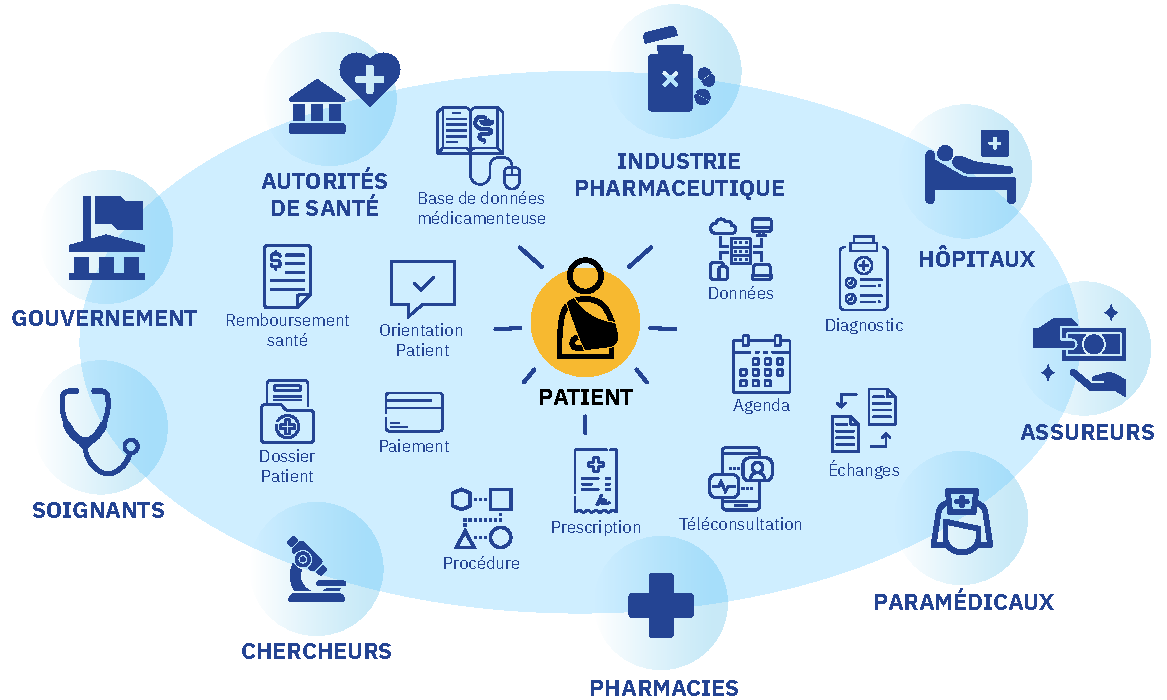
\includegraphics[width=\textwidth]{images/sec1/cegedim-ecosystem.pdf}
    \caption{Écosystème Cegedim}
\end{figure}
\subsubsection{Le Groupe Cegedim en quelques chiffres}
Cegedim compte près de 5 300 collaborateurs dans plus de 10 pays (voir figure ~\ref{fig:international_presence}) et a réalisé un chiffre d’affaires de 496.9 millions d’euros en 2020 \cite{cegedim-ca}.
Cegedim SA est cotée en bourse à Paris (EURONEXT : CGM).
\begin{figure}[H]
    \centering
    \begin{subfigure}[t]{0.3\textwidth}
    \centering
        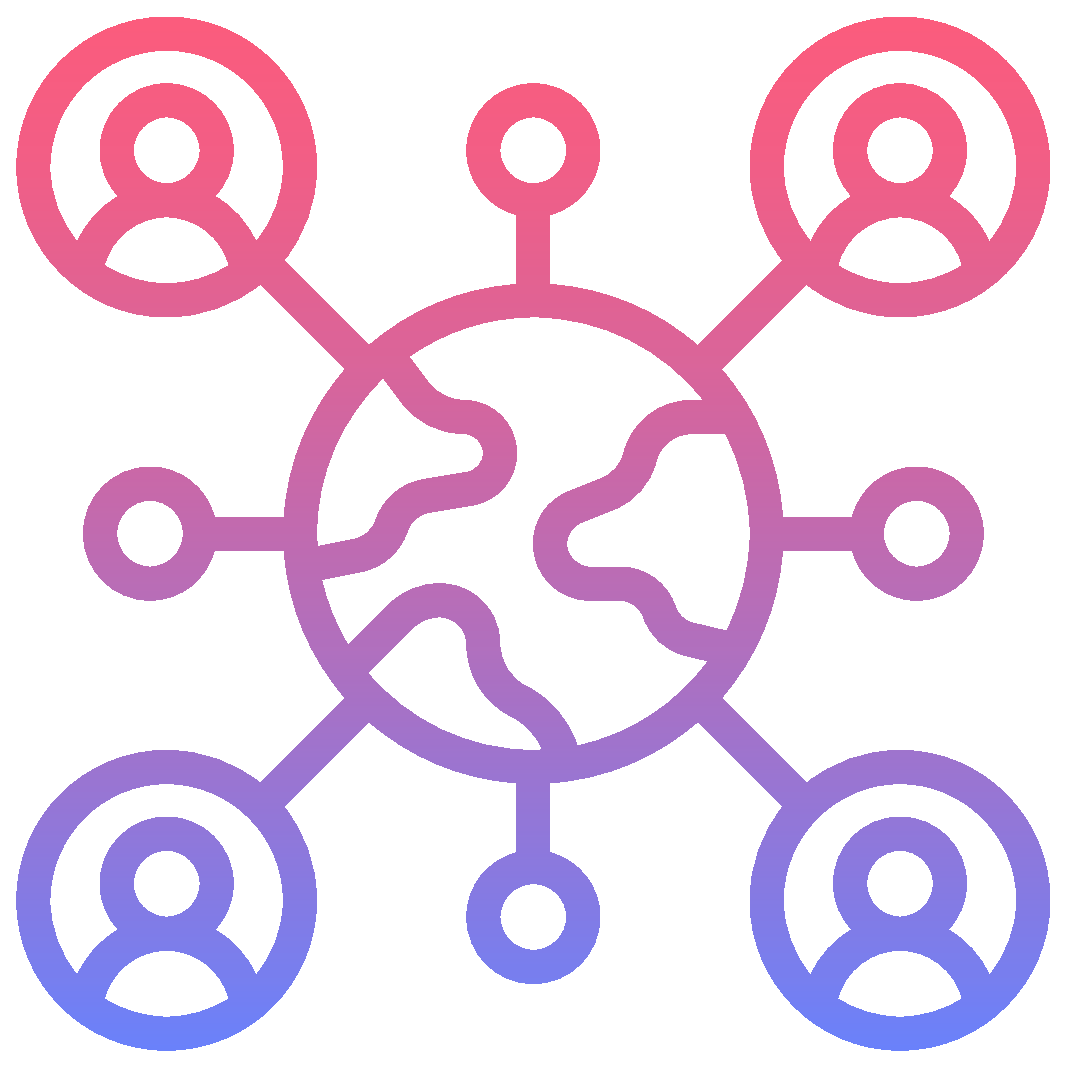
\includegraphics[height=0.28\textwidth]{images/sec1/social-network (1).pdf}
        \caption*{\centering + de \textbf{5 300} collaborateurs}
    \end{subfigure}
   \par\bigskip
    \begin{subfigure}[t]{0.3\textwidth}
    \centering
        
\includegraphics[height=0.28\textwidth]{images/sec1/connection.pdf}
        \caption*{Présence dans + de \textbf{10} pays}
    \end{subfigure}
    \hfill
    \begin{subfigure}[t]{0.3\textwidth}
    \centering
        
\includegraphics[height=0.28\textwidth]{images/sec1/medal (1).pdf}
        \caption*{\centering \textbf{Top 10} des éditeurs de logiciels français\protect\footnotemark}
    \end{subfigure}
    \hfill
    \begin{subfigure}[t]{0.3\textwidth}
    \centering
        
\includegraphics[height=0.26\textwidth]{images/sec1/analytics-market.pdf}
        \caption*{\centering Coté à la \textbf{Bourse} de Paris}
    \end{subfigure}
    \par\bigskip
    \begin{subfigure}[t]{0.3\textwidth}
    \begin{center}
        
\includegraphics[height=0.28\textwidth]{images/sec1/ca.pdf}
        \caption*{\centering \textbf{497 M€} de chiffre d’affaires}
    \end{center}
    \end{subfigure}
    \begin{subfigure}[t]{0.3\textwidth}
    \centering
        
\includegraphics[height=0.28\textwidth]{images/sec1/data-center.pdf}
        \caption*{\textbf{9} Datacenters}
    \end{subfigure}
    \caption{Groupe Cegedim en chiffres}
    \label{fig:subfigures}
\end{figure}
\footnotetext{Réalisé à partir d’une enquête par questionnaire en ligne. Le Palmarès a été réalisé sur la base des données transmises par chaque entreprise participante, et complétées dans certains cas par des sources extérieures. Certaines données, de nature confidentielle, sont traitées uniquement de façon agrégée. Lire le classement complet sur le site \href{https://www.truffle100.fr/2021.html}{Truffle 100} (publié le 8 juillet 2021).}
\begin{figure}[htb!]
    \centering
    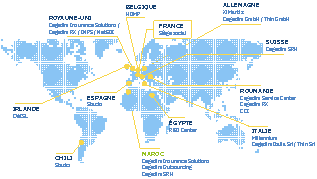
\includegraphics[width=\textwidth]{images/sec1/cegedim-presence-mondiale.pdf}
    \caption{Présence mondiale du groupe cegedim}
    \label{fig:international_presence}
\end{figure}

\subsubsection{Domaines d'activité}
Alliant maîtrise technologique des données, du numérique et des réseaux, les activités du groupe Cegedim se déclinent autour de \textbf{quatre divisions} opérationnelles. Ce découpage vise à améliorer la compréhension des activités en mettant en évidence les différents métiers exercés pour lesquels le lecteur disposera aisément de comparables connus sur le marché.\newline
\fboxsep=10pt\relax\fboxrule=2pt\relax%

\specialbox{white}{actBlue}{40pt}{0.50\textwidth}{
\begin{center}
  
\includegraphics[width=0.25\textwidth]{images/sec1/logiciels-et-services.pdf}  
\end{center}
{\footnotesize
regroupe l’ensemble des offres logiciels du Groupe sous toutes leurs formes (licence, SaaS, services internet) ainsi que l’hébergement (agrément HDS) et l‘infogérance. Cegedim cible l’assurance santé et prévoyance (France et Royaume-Uni), les professions paramédicales : kinésithérapeutes, infirmiers, orthophonistes, orthoptistes, podologues, sages-femmes… (France), les directions des ressources humaines (France), les pharmacies indépendantes, groupements ou chaînes de pharmacies (France, Roumanie et Royaume-Uni), les médecins et centres de santé (France, Royaume-Uni, Belgique, Espagne, Italie)\\\\}
\begin{tblr}
{ 
 rows = {bg=azure9},
 colsep=4pt,
 abovesep=4pt,
 row{2}={abovesep={8pt}},
 colspec={Q[r]Q[l]},
 rowspec={Q[m]Q[m]},
 vline{2} = {2pt,actBlue},
 }
{\Large \textcolor{actBlue}{\textbf{ 277,2 M€}}} &  CA 2020 \\
{\Large \textcolor{actBlue}{\textbf{ 55,8\%}}} &  CA groupe
\end{tblr}
}
\specialbox{white}{actPurple}{40pt}{0.50\textwidth}{
\begin{center}

\includegraphics[width=0.25\textwidth]{images/sec1/data-and-marketing.pdf}
\end{center}
{\footnotesize
regroupe les activités :
\begin{itemize}[itemsep=6pt]
    \item Données pour les autorités de santé, les professionnels de santé, les chercheurs, l’industrie de santé et ses partenaires en France, Italie, Allemagne, Espagne, Roumanie et Royaume-Uni ;
    \item Communication en pharmacie et parapharmacie d’enseigne en France sous format papier et numérique ;
    \item Marketing digital auprès des médecins ;
    \item Distribution de produits de santé.\\\\
\end{itemize}
}
\begin{tblr}
{ 
 rows = {bg=violet9},
 colsep=4pt,
 abovesep=4pt,
 row{2}={abovesep={8pt}},
 colspec={Q[r]Q[l]},
 rowspec={Q[m]Q[m]},
 vline{2} = {2pt,actPurple},
 }
{\Large \textcolor{actPurple}{\textbf{ 87,8 M€}}} &  CA 2020 \\
{\Large \textcolor{actPurple}{\textbf{ 17,7\%}}} &  CA groupe
\end{tblr}
}
\specialbox[t]{white}{actGreen}{40pt}{0.50\textwidth}{
\begin{center}

\includegraphics[width=0.25\textwidth]{images/sec1/flux.pdf}
\end{center}
{\footnotesize
regroupe les activités de gestion du tiers payant (France), de dématérialisation de processus et factures, d’archivage à valeur probante et d’EDI (France, Royaume-Uni, Allemagne). Pour cette activité Cegedim dispose de centres de services en France, Roumanie et Maroc.\\\\}
\begin{tblr}
{ 
 rows = {bg=teal9!50!white},
 colsep=4pt,
 abovesep=4pt,
 row{2}={abovesep={8pt}},
 colspec={Q[r]Q[l]},
 rowspec={Q[m]Q[m]},
 vline{2} = {2pt,actGreen},
 }
{\Large \textcolor{actGreen}{\textbf{ 79,4 M€}}} &  CA 2020 \\
{\Large \textcolor{actGreen}{\textbf{ 16,0\%}}} &  CA groupe
\end{tblr}}
\specialbox{white}{actPink}{40pt}{0.50\textwidth}{
\begin{center}
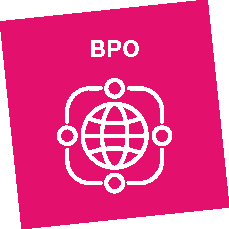
\includegraphics[width=0.25\textwidth]{images/sec1/BPO.pdf}
\end{center}
{\footnotesize
  regroupe les activités de Business Process Outsourcing en France pour le compte des assureurs complémentaires santé (entre autre gestion des remboursements) et institutions de prévoyance, et départements RH. Pour cette activité Cegedim dispose de centres de services en France et en Roumanie.\\\\}
  \begin{tblr}
{ 
 rows = {bg=purple9},
 colsep=4pt,
 abovesep=4pt,
 row{2}={abovesep={8pt}},
 colspec={Q[r]Q[l]},
 rowspec={Q[m]Q[m]},
 vline{2} = {2pt,actPink},
 }
{\Large \textcolor{actPink}{\textbf{ 48,9 M€}}} &  CA 2020 \\
{\Large \textcolor{actPink}{\textbf{ 9,8\%}}} &  CA groupe
\end{tblr}
 }
\par\bigskip
\begin{beware}[title=Note : ]
Cette ventilation par division présentée ci-dessus est la typologie privilégiée dans les communiqués de presse et les présentations financières de Cegedim. Il existe encore une cinquième division (non présentée ci-dessus), il s'agit de la division \textbf{Corporate et autres} et regroupe à la fois des activités inhérentes au statut de tête de Groupe coté, et des activités de support aux divisions du Groupe.
Cette division a réalisé en 2020 un chiffre d'affaires de 3,7 millions d'euros
(0,7\% du chiffre d'affaires consolidé du groupe). 

\end{beware}
\subsection{Cegedim SRH}
\subsubsection{Présentation}
Cegedim SRH, filiale du Groupe Cegedim, est l'un des leaders français des solutions et services de gestion de la paie et des ressources humaines. Acteur majeur du Cloud RH et des services externalisés, 
Cegedim SRH dispose d'une expertise de plus de 25 ans dans ce domaine accumulée et reflétée dans sa plateforme \textbf{TEAMS\textsuperscript{RH}} qui offre une large couverture fonctionnelle de solutions dédiées aux Ressources Humaines.\\
\begin{figure}[H]
    \centering
    
\includegraphics[width=0.25\textwidth]{images/sec1/cegedim-srh.pdf}
    \caption{Logo Cegedim SRH}
\end{figure}
La société compte parmi ses clients des entreprises nationales et internationales, de tous secteurs d’activité, issues des grands comptes et du mid-market.
\begin{figure}[H]
    \centering
    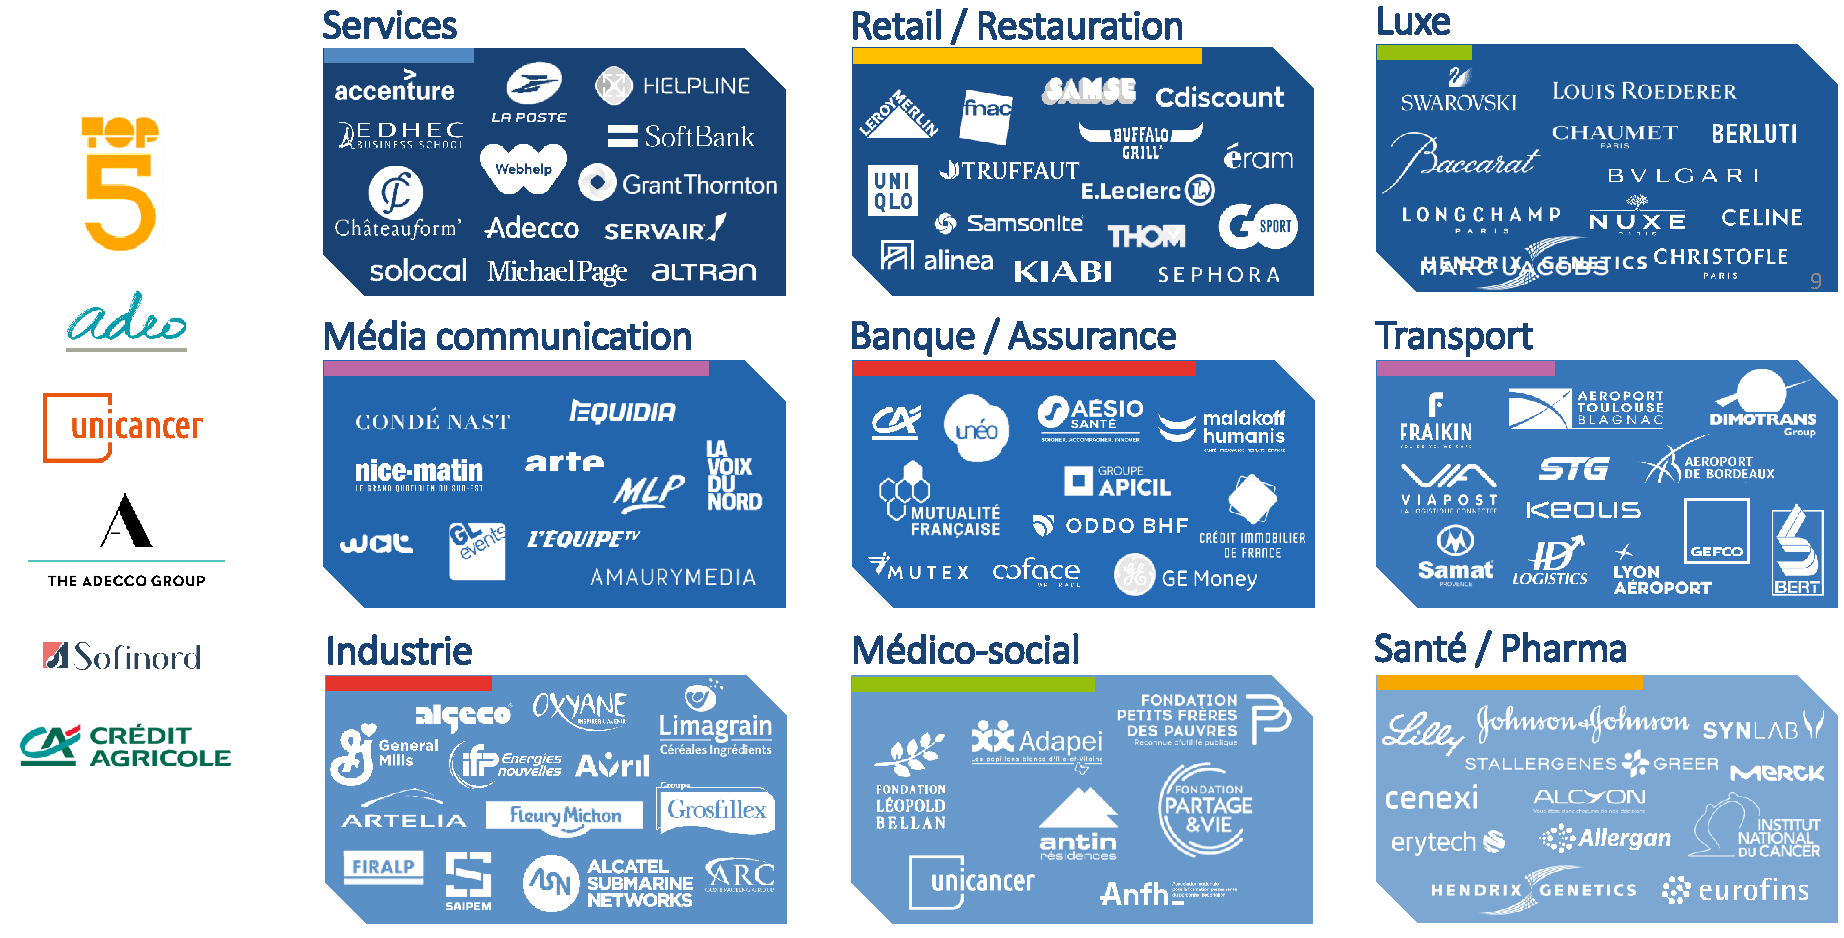
\includegraphics[width=\textwidth]{images/sec1/clients-cegedim-srh.pdf}
    \caption{Clients Cegedim SRH}
\end{figure}
\subsubsection{Domaines fonctionnels}
Capitalisant sur l'apport des nouvelles technologies, Cegedim SRH s'appuie sur un investissement continu et une stratégie de différenciation pour réinventer les outils de gestion RH à travers son offre TEAMS\textsuperscript{RH}, un SIRH complet et modulaire de solutions et services en mode externalisé pour répondre aux besoins d'agilité, de fiabilité et de performance de ses clients.
La plateforme TEAMS\textsuperscript{RH} est constituée d'un ensemble de modules tels que :

\begin{itemize}
    \item paie et gestion administrative,
    \item portail RH collaboratif,
    \item gestion des temps et des activités,
    \item pilotage social,
    \item gestion des RH (Entretiens et Formations),
    \item processus RH dématérialisés intégrés dans la solution (signature électronique et coffres-forts numériques).
\end{itemize}
\newpage
Pour aider ses clients à améliorer la performance de leurs activités, Cegedim SRH propose des services de gestion de la paie et des RH selon quatre niveaux de prestations, en fonction du degré de responsabilité de chaque acteur :\\ 

\vspace*{\fill}
\specialbox{white}{azure5}{40pt}{0.9\textwidth}{
{
\square{azure9}
\color{azure5}
\textbf{SaaS +}\\\\
}
abonnement aux services hébergés de TEAMS\textsuperscript{RH} incluant la maintenance corrective et les mises à jour légales et conventionnelles de l’application.\\}
\par\bigskip
\specialbox{white}{azure5}{40pt}{0.9\textwidth}{
{
\square{azure9} \square{azure8}
\color{azure5}
\textbf{Processing}\\\\
}
externalisation partielle avec pilotage de la relation client, le suivi du traitement de la paie, des opérations d’exploitation, de production et d’éditique.\\}
\par\bigskip
\specialbox{white}{azure5}{40pt}{0.9\textwidth}{
{
\square{azure9} \square{azure8} \square{azure7} 
\color{azure5}
\textbf{BPO on demand}\\\\
}
service d'externalisation de la paie évolutif et sur-mesure.\\}
\par\bigskip
\specialbox[t]{white}{azure5}{40pt}{0.9\textwidth}{
{
\square{azure9} \square{azure8} \square{azure7} \square{azure6}
\color{azure5}
\textbf{BPO}\\\\
}
externalisation complète avec prise en charge de l’ensemble des opérations de traitement de la paie (accréditation ISAE 3402).\\}
\vspace*{\fill}
\clearpage
\subsubsection{Agences et centres de services}
Cegedim SRH dispose de sites de proximité à Paris, Lyon, Lille, Nantes et Toulouse, associés à des centres de développement nearshore à Montargis, Vichy et Genève, et offshore à Bucarest et Rabat (voir figure ~\ref{fig:sites_cegedim}).
\begin{figure}[H]
    \centering
    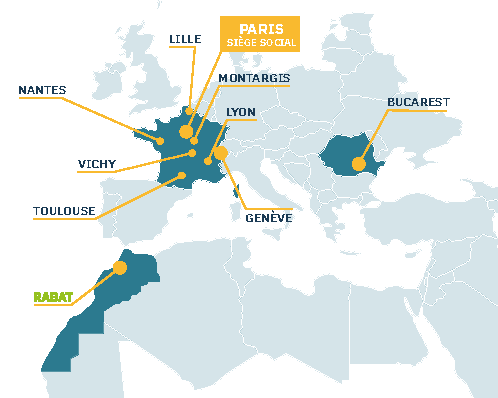
\includegraphics[width=0.78\textwidth]{images/sec1/cegedim-srh-map2.pdf}
    \caption{Les différents sites SRH}
    \label{fig:sites_cegedim}
\end{figure}
\subsubsection{Organigramme SRH}
Cegedim SRH dispose d’un organigramme qui montre sa structure générale ainsi que l’organisation de ses directions.
\tikzset{
        basic/.style={draw=none, text width=12em, rectangle,font=\bfseries, inner sep=0.25cm, outer sep=0cm,rounded corners=3pt},
        titre/.style={basic, align=center, minimum height=4em, text=azure3, fill=white,draw},
        objectif/.style={basic, align=center, anchor=north, text width=7.5em, minimum height=4.375em, text=azure3, fill=azure9, font=\footnotesize},
        specification/.style={basic, align=left, anchor=center, fill=alice, text width=6.25em, minimum height=3em,text=hoki,font=\footnotesize\bfseries}
    }

\begin{figure}[H]
\centering
 \resizebox{\linewidth}{!}{
   \begin{tikzpicture}[level distance=6em,line width=1pt,gray9,level 1/.style={sibling distance=10em},
    edge from parent path={(\tikzparentnode.south) |- (0em,2em) -| (\tikzchildnode.north)},
    edge from parent/.style={draw},on grid,node distance=2.25cm
    ]% <----- New options on grid and node distance
        \node [titre] {Cegedim SRH}
            child {node [objectif] (o1) {\textbf{Offre et R\&D}}}
            child {node [objectif] (o2) {\textbf{Développement commercial}}}
            child {node [objectif] (o3) {\textbf{Opérations}}}
            child {node [objectif] (o4) {\textbf{Externalisation de services et des TPE/PME}}}
            child {node [objectif] (o5) {\textbf{Satisfaction client et contrôle interne}}}
        ;
        \begin{scope}[every node/.style=specification]
            \node [below=of o1] (o11) {Offre};
            \node [below=of o11] (o12) {Développement technique};
            \node [below=of o12] (o13) {Fonctionnel Paie et\\Juridique};
            \node [below=of o13] (o14) {Fonctionnel RH};
            \node [below=of o14] (o15) {Technique et dev spécifiques};
            \node [below=of o15] (o16) {Qualité \&\\ Documentation};
            \node [below=of o2] (o21) {Marketing\\opérationnel};
            \node [below=of o21] (o22) {Avant-vente};
            \node [below=of o22] (o23) {Chasse};
            \node [below=of o23] (o24) {Parc};
            \node [below=of o3] (o31) {Boulogne};
            \node [below=of o31] (o32) {Lyon};
            \node [below=of o32] (o33) {Nantes};
            \node [below=of o33] (o34) {Lille};
            \node [below=of o34] (o35) {Toulouse};
            \node [below=of o35] (o36) {Centre de \\services};
            \node [below=of o4] (o41) {Rue de la Paye};
            \node [below=of o41] (o42) {BPO Bucarest};
            \node [below=of o42] (o43) {BPO/TPO\\Montargis et Boulogne};
            \node [below=of o43] (o44) {BPO Vichy};
            \node [below=of o44] (o45) {Projets TPO};
            \node [below=of o5] (o51) {Formation};
            \node [below=of o51] (o52) {AMOA et\\Assistance};
            \node [below=of o52] (o53) {RH};
            \node [below=of o53] (o54) {OPEX};
            \node [below=of o54] (o55) {Finances};
            \node [below=of o55] (o56) {Fabex};
        \end{scope}
        \foreach \value in {1,...,6}
            \draw (o1.west) -- ++(-0.5em,0em) |- (o1\value.west);
        \foreach \value in {1,...,4}
            \draw (o2.west) -- ++(-0.5em,0em) |- (o2\value.west);
        \foreach \value in {1,...,6}
            \draw (o3.west) -- ++(-0.5em,0em) |- (o3\value.west);
        \foreach \value in {1,...,5}
            \draw (o4.west) -- ++(-0.5em,0em) |- (o4\value.west);
        \foreach \value in {1,...,6}
            \draw (o5.west) -- ++(-0.5em,0em) |- (o5\value.west);
    \end{tikzpicture}
}
    \caption{Organigramme des Directions Cegedim SRH au 1er janvier 2019}
    \label{fig:organigramme_cegedim_srh}
\end{figure}